% Options for packages loaded elsewhere
\PassOptionsToPackage{unicode}{hyperref}
\PassOptionsToPackage{hyphens}{url}
%
\documentclass[
  letterpaper,
]{book}

\usepackage{amsmath,amssymb}
\usepackage{iftex}
\ifPDFTeX
  \usepackage[T1]{fontenc}
  \usepackage[utf8]{inputenc}
  \usepackage{textcomp} % provide euro and other symbols
\else % if luatex or xetex
  \usepackage{unicode-math}
  \defaultfontfeatures{Scale=MatchLowercase}
  \defaultfontfeatures[\rmfamily]{Ligatures=TeX,Scale=1}
\fi
\usepackage{lmodern}
\ifPDFTeX\else  
    % xetex/luatex font selection
\fi
% Use upquote if available, for straight quotes in verbatim environments
\IfFileExists{upquote.sty}{\usepackage{upquote}}{}
\IfFileExists{microtype.sty}{% use microtype if available
  \usepackage[]{microtype}
  \UseMicrotypeSet[protrusion]{basicmath} % disable protrusion for tt fonts
}{}
\makeatletter
\@ifundefined{KOMAClassName}{% if non-KOMA class
  \IfFileExists{parskip.sty}{%
    \usepackage{parskip}
  }{% else
    \setlength{\parindent}{0pt}
    \setlength{\parskip}{6pt plus 2pt minus 1pt}}
}{% if KOMA class
  \KOMAoptions{parskip=half}}
\makeatother
\usepackage{xcolor}
\setlength{\emergencystretch}{3em} % prevent overfull lines
\setcounter{secnumdepth}{5}
% Make \paragraph and \subparagraph free-standing
\makeatletter
\ifx\paragraph\undefined\else
  \let\oldparagraph\paragraph
  \renewcommand{\paragraph}{
    \@ifstar
      \xxxParagraphStar
      \xxxParagraphNoStar
  }
  \newcommand{\xxxParagraphStar}[1]{\oldparagraph*{#1}\mbox{}}
  \newcommand{\xxxParagraphNoStar}[1]{\oldparagraph{#1}\mbox{}}
\fi
\ifx\subparagraph\undefined\else
  \let\oldsubparagraph\subparagraph
  \renewcommand{\subparagraph}{
    \@ifstar
      \xxxSubParagraphStar
      \xxxSubParagraphNoStar
  }
  \newcommand{\xxxSubParagraphStar}[1]{\oldsubparagraph*{#1}\mbox{}}
  \newcommand{\xxxSubParagraphNoStar}[1]{\oldsubparagraph{#1}\mbox{}}
\fi
\makeatother

\usepackage{color}
\usepackage{fancyvrb}
\newcommand{\VerbBar}{|}
\newcommand{\VERB}{\Verb[commandchars=\\\{\}]}
\DefineVerbatimEnvironment{Highlighting}{Verbatim}{commandchars=\\\{\}}
% Add ',fontsize=\small' for more characters per line
\usepackage{framed}
\definecolor{shadecolor}{RGB}{241,243,245}
\newenvironment{Shaded}{\begin{snugshade}}{\end{snugshade}}
\newcommand{\AlertTok}[1]{\textcolor[rgb]{0.68,0.00,0.00}{#1}}
\newcommand{\AnnotationTok}[1]{\textcolor[rgb]{0.37,0.37,0.37}{#1}}
\newcommand{\AttributeTok}[1]{\textcolor[rgb]{0.40,0.45,0.13}{#1}}
\newcommand{\BaseNTok}[1]{\textcolor[rgb]{0.68,0.00,0.00}{#1}}
\newcommand{\BuiltInTok}[1]{\textcolor[rgb]{0.00,0.23,0.31}{#1}}
\newcommand{\CharTok}[1]{\textcolor[rgb]{0.13,0.47,0.30}{#1}}
\newcommand{\CommentTok}[1]{\textcolor[rgb]{0.37,0.37,0.37}{#1}}
\newcommand{\CommentVarTok}[1]{\textcolor[rgb]{0.37,0.37,0.37}{\textit{#1}}}
\newcommand{\ConstantTok}[1]{\textcolor[rgb]{0.56,0.35,0.01}{#1}}
\newcommand{\ControlFlowTok}[1]{\textcolor[rgb]{0.00,0.23,0.31}{\textbf{#1}}}
\newcommand{\DataTypeTok}[1]{\textcolor[rgb]{0.68,0.00,0.00}{#1}}
\newcommand{\DecValTok}[1]{\textcolor[rgb]{0.68,0.00,0.00}{#1}}
\newcommand{\DocumentationTok}[1]{\textcolor[rgb]{0.37,0.37,0.37}{\textit{#1}}}
\newcommand{\ErrorTok}[1]{\textcolor[rgb]{0.68,0.00,0.00}{#1}}
\newcommand{\ExtensionTok}[1]{\textcolor[rgb]{0.00,0.23,0.31}{#1}}
\newcommand{\FloatTok}[1]{\textcolor[rgb]{0.68,0.00,0.00}{#1}}
\newcommand{\FunctionTok}[1]{\textcolor[rgb]{0.28,0.35,0.67}{#1}}
\newcommand{\ImportTok}[1]{\textcolor[rgb]{0.00,0.46,0.62}{#1}}
\newcommand{\InformationTok}[1]{\textcolor[rgb]{0.37,0.37,0.37}{#1}}
\newcommand{\KeywordTok}[1]{\textcolor[rgb]{0.00,0.23,0.31}{\textbf{#1}}}
\newcommand{\NormalTok}[1]{\textcolor[rgb]{0.00,0.23,0.31}{#1}}
\newcommand{\OperatorTok}[1]{\textcolor[rgb]{0.37,0.37,0.37}{#1}}
\newcommand{\OtherTok}[1]{\textcolor[rgb]{0.00,0.23,0.31}{#1}}
\newcommand{\PreprocessorTok}[1]{\textcolor[rgb]{0.68,0.00,0.00}{#1}}
\newcommand{\RegionMarkerTok}[1]{\textcolor[rgb]{0.00,0.23,0.31}{#1}}
\newcommand{\SpecialCharTok}[1]{\textcolor[rgb]{0.37,0.37,0.37}{#1}}
\newcommand{\SpecialStringTok}[1]{\textcolor[rgb]{0.13,0.47,0.30}{#1}}
\newcommand{\StringTok}[1]{\textcolor[rgb]{0.13,0.47,0.30}{#1}}
\newcommand{\VariableTok}[1]{\textcolor[rgb]{0.07,0.07,0.07}{#1}}
\newcommand{\VerbatimStringTok}[1]{\textcolor[rgb]{0.13,0.47,0.30}{#1}}
\newcommand{\WarningTok}[1]{\textcolor[rgb]{0.37,0.37,0.37}{\textit{#1}}}

\providecommand{\tightlist}{%
  \setlength{\itemsep}{0pt}\setlength{\parskip}{0pt}}\usepackage{longtable,booktabs,array}
\usepackage{calc} % for calculating minipage widths
% Correct order of tables after \paragraph or \subparagraph
\usepackage{etoolbox}
\makeatletter
\patchcmd\longtable{\par}{\if@noskipsec\mbox{}\fi\par}{}{}
\makeatother
% Allow footnotes in longtable head/foot
\IfFileExists{footnotehyper.sty}{\usepackage{footnotehyper}}{\usepackage{footnote}}
\makesavenoteenv{longtable}
\usepackage{graphicx}
\makeatletter
\newsavebox\pandoc@box
\newcommand*\pandocbounded[1]{% scales image to fit in text height/width
  \sbox\pandoc@box{#1}%
  \Gscale@div\@tempa{\textheight}{\dimexpr\ht\pandoc@box+\dp\pandoc@box\relax}%
  \Gscale@div\@tempb{\linewidth}{\wd\pandoc@box}%
  \ifdim\@tempb\p@<\@tempa\p@\let\@tempa\@tempb\fi% select the smaller of both
  \ifdim\@tempa\p@<\p@\scalebox{\@tempa}{\usebox\pandoc@box}%
  \else\usebox{\pandoc@box}%
  \fi%
}
% Set default figure placement to htbp
\def\fps@figure{htbp}
\makeatother
% definitions for citeproc citations
\NewDocumentCommand\citeproctext{}{}
\NewDocumentCommand\citeproc{mm}{%
  \begingroup\def\citeproctext{#2}\cite{#1}\endgroup}
\makeatletter
 % allow citations to break across lines
 \let\@cite@ofmt\@firstofone
 % avoid brackets around text for \cite:
 \def\@biblabel#1{}
 \def\@cite#1#2{{#1\if@tempswa , #2\fi}}
\makeatother
\newlength{\cslhangindent}
\setlength{\cslhangindent}{1.5em}
\newlength{\csllabelwidth}
\setlength{\csllabelwidth}{3em}
\newenvironment{CSLReferences}[2] % #1 hanging-indent, #2 entry-spacing
 {\begin{list}{}{%
  \setlength{\itemindent}{0pt}
  \setlength{\leftmargin}{0pt}
  \setlength{\parsep}{0pt}
  % turn on hanging indent if param 1 is 1
  \ifodd #1
   \setlength{\leftmargin}{\cslhangindent}
   \setlength{\itemindent}{-1\cslhangindent}
  \fi
  % set entry spacing
  \setlength{\itemsep}{#2\baselineskip}}}
 {\end{list}}
\usepackage{calc}
\newcommand{\CSLBlock}[1]{\hfill\break\parbox[t]{\linewidth}{\strut\ignorespaces#1\strut}}
\newcommand{\CSLLeftMargin}[1]{\parbox[t]{\csllabelwidth}{\strut#1\strut}}
\newcommand{\CSLRightInline}[1]{\parbox[t]{\linewidth - \csllabelwidth}{\strut#1\strut}}
\newcommand{\CSLIndent}[1]{\hspace{\cslhangindent}#1}

\makeatletter
\@ifpackageloaded{tcolorbox}{}{\usepackage[skins,breakable]{tcolorbox}}
\@ifpackageloaded{fontawesome5}{}{\usepackage{fontawesome5}}
\definecolor{quarto-callout-color}{HTML}{909090}
\definecolor{quarto-callout-note-color}{HTML}{0758E5}
\definecolor{quarto-callout-important-color}{HTML}{CC1914}
\definecolor{quarto-callout-warning-color}{HTML}{EB9113}
\definecolor{quarto-callout-tip-color}{HTML}{00A047}
\definecolor{quarto-callout-caution-color}{HTML}{FC5300}
\definecolor{quarto-callout-color-frame}{HTML}{acacac}
\definecolor{quarto-callout-note-color-frame}{HTML}{4582ec}
\definecolor{quarto-callout-important-color-frame}{HTML}{d9534f}
\definecolor{quarto-callout-warning-color-frame}{HTML}{f0ad4e}
\definecolor{quarto-callout-tip-color-frame}{HTML}{02b875}
\definecolor{quarto-callout-caution-color-frame}{HTML}{fd7e14}
\makeatother
\makeatletter
\@ifpackageloaded{bookmark}{}{\usepackage{bookmark}}
\makeatother
\makeatletter
\@ifpackageloaded{caption}{}{\usepackage{caption}}
\AtBeginDocument{%
\ifdefined\contentsname
  \renewcommand*\contentsname{Table of contents}
\else
  \newcommand\contentsname{Table of contents}
\fi
\ifdefined\listfigurename
  \renewcommand*\listfigurename{List of Figures}
\else
  \newcommand\listfigurename{List of Figures}
\fi
\ifdefined\listtablename
  \renewcommand*\listtablename{List of Tables}
\else
  \newcommand\listtablename{List of Tables}
\fi
\ifdefined\figurename
  \renewcommand*\figurename{Figure}
\else
  \newcommand\figurename{Figure}
\fi
\ifdefined\tablename
  \renewcommand*\tablename{Table}
\else
  \newcommand\tablename{Table}
\fi
}
\@ifpackageloaded{float}{}{\usepackage{float}}
\floatstyle{ruled}
\@ifundefined{c@chapter}{\newfloat{codelisting}{h}{lop}}{\newfloat{codelisting}{h}{lop}[chapter]}
\floatname{codelisting}{Listing}
\newcommand*\listoflistings{\listof{codelisting}{List of Listings}}
\makeatother
\makeatletter
\makeatother
\makeatletter
\@ifpackageloaded{caption}{}{\usepackage{caption}}
\@ifpackageloaded{subcaption}{}{\usepackage{subcaption}}
\makeatother

\usepackage{bookmark}

\IfFileExists{xurl.sty}{\usepackage{xurl}}{} % add URL line breaks if available
\urlstyle{same} % disable monospaced font for URLs
\hypersetup{
  pdftitle={STA2020 ANOVA Notes},
  pdfauthor={Ané Cloete},
  hidelinks,
  pdfcreator={LaTeX via pandoc}}


\title{STA2020 ANOVA Notes}
\author{Ané Cloete}
\date{2024-12-17}

\begin{document}
\frontmatter
\maketitle

\renewcommand*\contentsname{Table of contents}
{
\setcounter{tocdepth}{2}
\tableofcontents
}

\mainmatter
\bookmarksetup{startatroot}

\chapter*{Preface}\label{preface}
\addcontentsline{toc}{chapter}{Preface}

\markboth{Preface}{Preface}

\emph{Welcome to the Experimental Design and ANOVA section of STA2020.}

This book is not an exhaustive guide to designing experiments or
conducting ANOVA. Instead, it has been tailored specifically to align
with the learning outcomes and methods covered in STA2020.

This module consists of four main sections:

\begin{enumerate}
\def\labelenumi{\arabic{enumi}.}
\tightlist
\item
  Experimental Design
\item
  Completely Randomized Designs
\item
  Randomized Complete Block Designs
\item
  Factorial Experiments
\end{enumerate}

The first two chapters lay the groundwork for the module. Once you grasp
these concepts, the remaining sections should be easier to follow.
Before diving into these topics, there are two preliminary sections:

\begin{enumerate}
\def\labelenumi{\arabic{enumi}.}
\tightlist
\item
  A brief introduction to statistical modeling
\item
  A guide to hypothesis testing
\end{enumerate}

I encourage you to read through these first, as they provide essential
context for the rest of the material.

Throughout the book, you will find R code presented in chunks like this:

\begin{Shaded}
\begin{Highlighting}[]
\NormalTok{x }\OtherTok{\textless{}{-}} \FunctionTok{c}\NormalTok{(}\DecValTok{1}\NormalTok{,}\DecValTok{2}\NormalTok{,}\DecValTok{3}\NormalTok{,}\DecValTok{4}\NormalTok{,}\DecValTok{5}\NormalTok{)}
\FunctionTok{mean}\NormalTok{(x) }\CommentTok{\# Computes the mean of a set of numbers  }
\end{Highlighting}
\end{Shaded}

\begin{verbatim}
[1] 3
\end{verbatim}

R is consistently used to visualize, illustrate, and demonstrate key
methods and concepts. Running the code yourself will greatly enhance
your understanding, so I encourage you to do so.

\begin{quote}
Some parts of these notes have been adapted from the STA1007 notes,
authored by Dr.~Res Altwegg and Dr.~Birgit Erni, as well as from various
textbooks.
\end{quote}

\bookmarksetup{startatroot}

\chapter*{Statistical Modelling}\label{statistical-modelling}
\addcontentsline{toc}{chapter}{Statistical Modelling}

\markboth{Statistical Modelling}{Statistical Modelling}

\section*{What is a Model?}\label{what-is-a-model}
\addcontentsline{toc}{section}{What is a Model?}

\markright{What is a Model?}

A \textbf{statistical model} is a mathematical representation of how
data is generated. It describes the relationship between observed data
and underlying factors (parameters) while accounting for random
variation. Suppose that we are interested in estimating the age of a
tree from its stem diameter. To do this we need to know by how much the
stem diameter increases per year. We could describe this relationship or
process as follows:

\[D = \alpha + \beta \times Age\] describing a linear increase of
diameter with age. Once we have a good idea of how fast diameter
increases with age (β) we can predict diameter from age. The
(mathematical) model above is a very simple representation of this
process with only two parameters, the intercept and the growth rate.

With the chosen parameter values, diameter increases linearly with age.
Of course, this model is not realistic except for special situations but
it gives us powerful insights. In reality we don't know \(\beta\), but
usually need to estimate it from data. Also, not every tree grows
equally fast, because of environmental and individual differences
between trees. We can accept that the above is a simple model for the
average behaviour of a tree, but to capture variability between trees
(because of variability between environmental conditions from tree to
tree, variability between individual trees, measurement error), we add
an error term.

\[D = \alpha + \beta \times Age_i + e_i\]

The response that we observe is then described by an average behaviour,
but the actual observed value will vary around this average. To
summarise, the statistical model has a stochastic component which
captures variability in the response that cannot be explained by the
deterministic part of the model. Another distinguishing feature of
statistical modelling is that we obtain estimates of the parameter
values from the data, e.g.~by fitting a line to the observations,
i.e.~we learn from data.

\section*{More generally}\label{more-generally}
\addcontentsline{toc}{section}{More generally}

\markright{More generally}

Statistical models are not perfect predictors of the data, rather they
attempt to describe the ``central tendency'' of the observations. To get
to the actual observed value some deviation from the central tendency
needs to added (i.e.~error). Such models typically have the following
the form:

\[
\text{Observed Response} = \text{Model Predicted Response} + \text{Error}
\]

Mathematically this can be stated as:

\[Y = \hat{Y} + e\]

A simple example of a statistical model you may have encountered is the
\textbf{mean} as a predictor. Suppose you measure the number of
customers entering two stores over 20 days. The observed counts for each
store fluctuate daily, but you may want to summarize the data using the
average number of customers.

For each store \(i\), a basic statistical model for these observations
would be:

\[
Y_{ij} = \mu_i + e_{ij}
\]

where:

\begin{itemize}
\tightlist
\item
  \(Y_{ij}\) is the number of customers observed on day \(j\) at store
  1,
\item
  \(\mu_i\) is the true mean number of customers at store \(i\),
\item
  \(e_{ij}\) is the error term, representing deviations from the mean.
\end{itemize}

The error term \(e_{ij}\) accounts for day-to-day fluctuations that
cause the actual number of customers to vary around the mean. Below this
data is simulated and plotted, with the model overlain. The black line
is the mean and the red dashed line represents the error for one
observation, i.e.~deviation from the fitted model response, in this case
the mean.

\begin{Shaded}
\begin{Highlighting}[]
\NormalTok{store1 }\OtherTok{\textless{}{-}} \FunctionTok{rpois}\NormalTok{(}\DecValTok{20}\NormalTok{, }\DecValTok{50}\NormalTok{)}
\NormalTok{store2 }\OtherTok{\textless{}{-}} \FunctionTok{rpois}\NormalTok{(}\DecValTok{20}\NormalTok{, }\DecValTok{15}\NormalTok{)}
\NormalTok{storedata }\OtherTok{\textless{}{-}} \FunctionTok{data.frame}\NormalTok{(}\AttributeTok{numcust =} \FunctionTok{c}\NormalTok{(store1, store2),}
                        \AttributeTok{store =} \FunctionTok{factor}\NormalTok{(}\FunctionTok{rep}\NormalTok{(}\FunctionTok{c}\NormalTok{(}\StringTok{"Store 1"}\NormalTok{, }\StringTok{"Store 2"}\NormalTok{), }\AttributeTok{each =} \DecValTok{20}\NormalTok{)))}

\FunctionTok{stripchart}\NormalTok{(numcust }\SpecialCharTok{\textasciitilde{}}\NormalTok{ store, }\AttributeTok{data =}\NormalTok{ storedata,}
           \AttributeTok{method =} \StringTok{"jitter"}\NormalTok{, }\AttributeTok{pch =} \DecValTok{16}\NormalTok{, }\AttributeTok{col =} \FunctionTok{c}\NormalTok{(}\StringTok{"deepskyblue"}\NormalTok{, }\StringTok{"orange"}\NormalTok{),}
           \AttributeTok{vertical =} \ConstantTok{TRUE}\NormalTok{, }\AttributeTok{main =} \StringTok{"Customer Counts per Store"}\NormalTok{,}
           \AttributeTok{xlab =} \StringTok{"Store"}\NormalTok{, }\AttributeTok{ylab =} \StringTok{"Number of Customers"}\NormalTok{)}
\NormalTok{means }\OtherTok{\textless{}{-}} \FunctionTok{tapply}\NormalTok{(storedata}\SpecialCharTok{$}\NormalTok{numcust, storedata}\SpecialCharTok{$}\NormalTok{store, mean)}
\FunctionTok{segments}\NormalTok{(}\AttributeTok{x0 =} \DecValTok{1}\SpecialCharTok{:}\DecValTok{2}\SpecialCharTok{{-}} \FloatTok{0.1}\NormalTok{, }\AttributeTok{x1 =} \DecValTok{1}\SpecialCharTok{:}\DecValTok{2} \SpecialCharTok{+} \FloatTok{0.1}\NormalTok{, }\AttributeTok{y0 =}\NormalTok{ means, }\AttributeTok{y1 =}\NormalTok{ means, }\AttributeTok{lwd =} \DecValTok{3}\NormalTok{, }\AttributeTok{col =} \StringTok{"black"}\NormalTok{) }
\NormalTok{min\_count }\OtherTok{\textless{}{-}} \FunctionTok{min}\NormalTok{(storedata}\SpecialCharTok{$}\NormalTok{numcust[storedata}\SpecialCharTok{$}\NormalTok{store }\SpecialCharTok{==} \StringTok{"Store 1"}\NormalTok{])}
\NormalTok{min\_x }\OtherTok{\textless{}{-}} \FunctionTok{jitter}\NormalTok{(}\FunctionTok{rep}\NormalTok{(}\DecValTok{1}\NormalTok{, }\FunctionTok{sum}\NormalTok{(storedata}\SpecialCharTok{$}\NormalTok{numcust }\SpecialCharTok{==}\NormalTok{ min\_count))) }
\FunctionTok{points}\NormalTok{(min\_x, min\_count, }\AttributeTok{col =} \StringTok{"red"}\NormalTok{, }\AttributeTok{pch =} \DecValTok{16}\NormalTok{, }\AttributeTok{cex =} \FloatTok{1.2}\NormalTok{) }
\FunctionTok{segments}\NormalTok{(}\AttributeTok{x0 =}\NormalTok{ min\_x, }\AttributeTok{x1 =}\NormalTok{ min\_x, }\AttributeTok{y0 =}\NormalTok{ min\_count, }\AttributeTok{y1 =}\NormalTok{ means[}\StringTok{"Store 1"}\NormalTok{], }\AttributeTok{col =} \StringTok{"red"}\NormalTok{, }\AttributeTok{lwd =} \DecValTok{2}\NormalTok{, }\AttributeTok{lty =} \DecValTok{2}\NormalTok{)}
\end{Highlighting}
\end{Shaded}

\pandocbounded{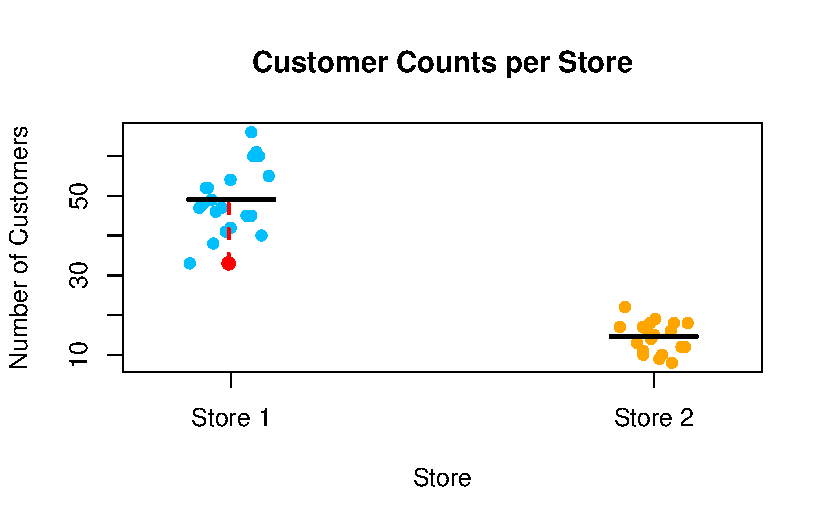
\includegraphics[keepaspectratio]{00_ModelConcepts_files/figure-pdf/unnamed-chunk-1-1.pdf}}

Another basic example of this structure is a \textbf{linear regression
model}:

\[
Y_i = \beta_0 + \beta_1 X_i + e_i
\]

where:

\begin{itemize}
\tightlist
\item
  \(Y_i\) is the observed response,
\item
  \(\beta_0\) and \(\beta_1\) are unknown parameters representing the
  intercept and slope,
\item
  \(X_i\) is the predictor variable,
\item
  \(e_i\) is the random error term.
\end{itemize}

\begin{Shaded}
\begin{Highlighting}[]
\CommentTok{\# Generate random x values and error term}
\FunctionTok{set.seed}\NormalTok{(}\DecValTok{123}\NormalTok{)  }\CommentTok{\# Ensures reproducibility}
\NormalTok{x }\OtherTok{\textless{}{-}} \FunctionTok{rnorm}\NormalTok{(}\DecValTok{35}\NormalTok{, }\AttributeTok{mean =} \DecValTok{35}\NormalTok{, }\AttributeTok{sd =} \DecValTok{5}\NormalTok{)}
\NormalTok{error }\OtherTok{\textless{}{-}} \FunctionTok{rnorm}\NormalTok{(}\DecValTok{35}\NormalTok{, }\AttributeTok{mean =} \DecValTok{0}\NormalTok{, }\AttributeTok{sd =} \DecValTok{5}\NormalTok{)}

\CommentTok{\# Define true model parameters}
\NormalTok{beta0 }\OtherTok{\textless{}{-}} \DecValTok{2}
\NormalTok{beta1 }\OtherTok{\textless{}{-}} \FloatTok{1.5}

\CommentTok{\# Generate y values based on the regression model}
\NormalTok{y }\OtherTok{\textless{}{-}}\NormalTok{ beta0 }\SpecialCharTok{+}\NormalTok{ beta1 }\SpecialCharTok{*}\NormalTok{ x }\SpecialCharTok{+}\NormalTok{ error}

\CommentTok{\# Fit a linear regression model}
\NormalTok{model }\OtherTok{\textless{}{-}} \FunctionTok{lm}\NormalTok{(y }\SpecialCharTok{\textasciitilde{}}\NormalTok{ x)  }\CommentTok{\# This was missing!}

\CommentTok{\# Select an observation to highlight}
\NormalTok{obs\_index }\OtherTok{\textless{}{-}} \DecValTok{20}  
\NormalTok{x\_obs }\OtherTok{\textless{}{-}}\NormalTok{ x[obs\_index]}
\NormalTok{y\_obs }\OtherTok{\textless{}{-}}\NormalTok{ y[obs\_index]}
\NormalTok{y\_pred }\OtherTok{\textless{}{-}} \FunctionTok{predict}\NormalTok{(model, }\AttributeTok{newdata =} \FunctionTok{data.frame}\NormalTok{(}\AttributeTok{x =}\NormalTok{ x\_obs))  }

\CommentTok{\# Scatter plot of data points}
\FunctionTok{plot}\NormalTok{(x, y, }\AttributeTok{pch =} \DecValTok{16}\NormalTok{, }\AttributeTok{col =} \StringTok{"darkseagreen"}\NormalTok{,}
     \AttributeTok{xlab =} \StringTok{"X"}\NormalTok{, }\AttributeTok{ylab =} \StringTok{"Y"}\NormalTok{,}
     \AttributeTok{main =} \StringTok{"Scatter Plot with Regression Line"}\NormalTok{,}
     \AttributeTok{cex.lab =} \FloatTok{1.5}\NormalTok{, }\AttributeTok{cex.axis =} \FloatTok{1.2}\NormalTok{, }\AttributeTok{cex.main =} \FloatTok{1.5}\NormalTok{)}

\CommentTok{\# Add regression line}
\FunctionTok{abline}\NormalTok{(model, }\AttributeTok{col =} \StringTok{"black"}\NormalTok{, }\AttributeTok{lwd =} \DecValTok{2}\NormalTok{)}

\CommentTok{\# Highlight the observed point}
\FunctionTok{points}\NormalTok{(x\_obs, y\_obs, }\AttributeTok{col =} \StringTok{"red"}\NormalTok{, }\AttributeTok{pch =} \DecValTok{16}\NormalTok{, }\AttributeTok{cex =} \FloatTok{1.2}\NormalTok{)  }

\CommentTok{\# Draw a dashed vertical line from the predicted value to the observed value}
\FunctionTok{segments}\NormalTok{(}\AttributeTok{x0 =}\NormalTok{ x\_obs, }\AttributeTok{x1 =}\NormalTok{ x\_obs, }\AttributeTok{y0 =}\NormalTok{ y\_pred, }\AttributeTok{y1 =}\NormalTok{ y\_obs, }\AttributeTok{col =} \StringTok{"red"}\NormalTok{, }\AttributeTok{lwd =} \DecValTok{2}\NormalTok{, }\AttributeTok{lty =} \DecValTok{2}\NormalTok{)}
\end{Highlighting}
\end{Shaded}

\pandocbounded{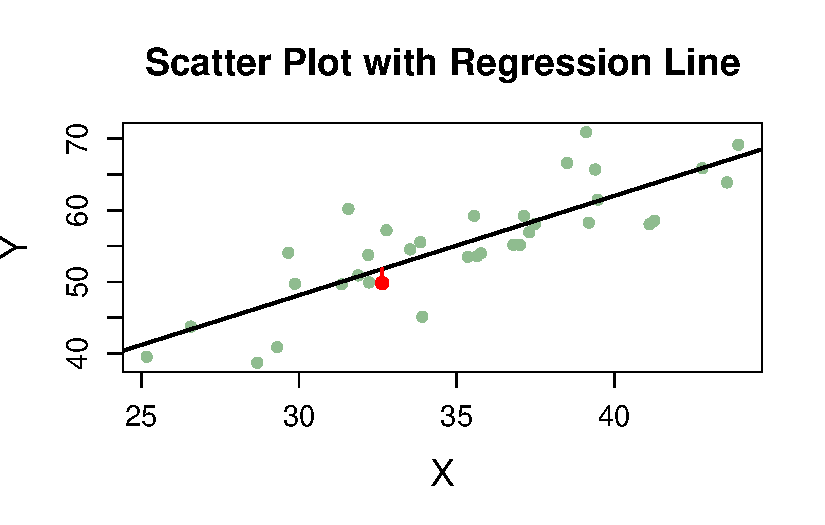
\includegraphics[keepaspectratio]{00_ModelConcepts_files/figure-pdf/unnamed-chunk-2-1.pdf}}

\section*{Notation}\label{notation}
\addcontentsline{toc}{section}{Notation}

\markright{Notation}

When we fit the model to our data, we \textbf{estimate} the unknown
parameters using observed data. We denote these estimates using
\textbf{hat notation} to distinguish them from the true (but unknown)
population parameters:

\[
\hat{\beta}_0, \quad \hat{\beta}_1
\]

Similarly, the \textbf{fitted values} (model-predicted responses) are
denoted as:

\[
\hat{Y}_i = \hat{\beta}_0 + \hat{\beta}_1 X_i.
\]

Thus, after fitting the model, the observed response can be rewritten
as:

\[
Y_i = (\hat{\beta}_0 + \hat{\beta}_1 X_i) + e_i = \hat{Y}_i + e_i
\]

where:

\begin{itemize}
\tightlist
\item
  \(\hat{Y}_i\) is the \textbf{fitted (predicted) value}, and
\item
  \(e_i = Y_i - \hat{Y}_i\) is the \textbf{residual}, representing the
  difference between the observed and predicted values.
\end{itemize}

\bookmarksetup{startatroot}

\chapter*{A brief guideline to hypothesis
testing}\label{a-brief-guideline-to-hypothesis-testing}
\addcontentsline{toc}{chapter}{A brief guideline to hypothesis testing}

\markboth{A brief guideline to hypothesis testing}{A brief guideline to
hypothesis testing}

\begin{quote}
These notes have been adapted from the STA1007 notes (authored by Dr Res
Altwegg and Dr Greg Distiller and some other textbooks.
\end{quote}

Hypothesis testing is a statistical procedure of using sample data to
make inferences about populations. Unlike estimation, where the goal is
to quantify a parameter, hypothesis testing assesses whether an observed
effect is statistically significant. More specifically, a hypothesis
test evaluates two mutually exclusive statements about the population
and determines which statement the data supports.

\subsection*{The General Framework}\label{the-general-framework}
\addcontentsline{toc}{subsection}{The General Framework}

Hypothesis testing follows a structured process:

\begin{enumerate}
\def\labelenumi{\arabic{enumi}.}
\tightlist
\item
  \textbf{State the Hypotheses}: Define the null hypothesis (H₀) and the
  alternative hypothesis (H₁).
\end{enumerate}

The basic idea of hypothesis testing is that we set up a so-called null
hypothesis and then ask how likely our data are if the null hypothesis
were true. If they are unlikely, we conclude that we have found evidence
against the null hypothesis, i.e.~the null hypothesis is probably not
true.

The alternative hypothesis covers all the possibilities not covered by
the null hypothesis. If we conclude that the null hypothesis is probably
not true, that means that the alternative hypothesis is probably true.
These two hypotheses are not equal in how we treat them:

\begin{itemize}
\item
  We start by assuming the null is true and check if the data gives
  enough evidence to reject it.
\item
  If the data strongly contradicts the null, we lean toward the
  alternative hypothesis.
\end{itemize}

But we never prove the alternative hypothesis outright---we only show
that the null is unlikely based on the evidence. You can think of the
null hypothesis as representing a baseline against which the data are
compared, whereas the alternative hypothesis is what we really care
about, worry about or want to demonstrate. This is an important
asymmetry and will need some careful reflection.

Below is an example:

Null Hypothesis (\(H_0\)): ``The average weight of chocolate bars is
100g.''

Alternative Hypothesis (\(H_A\)): ``The average weight of chocolate bars
is less than 100g.''

Lack of evidence against \(H_0\) is not the same as evidence for
\(H_0\). We never say that we have evidence for \(H_0\) or that we
accept \(H_0\) as true.

\begin{enumerate}
\def\labelenumi{\arabic{enumi}.}
\setcounter{enumi}{1}
\tightlist
\item
  \textbf{Choose a Test Statistic}: Select an appropriate statistic to
  measure the observed effect.
\end{enumerate}

A numerical function of the data that quantifies the strength of the
observed effect, whose value determines the result of the test. Examples
include the mean difference, proportion difference, or z-score.

\begin{enumerate}
\def\labelenumi{\arabic{enumi}.}
\setcounter{enumi}{2}
\tightlist
\item
  \textbf{Determine the Null Distribution:} Establish what the test
  statistic would look like if H₀ were true.
\end{enumerate}

We have a test statistic and to say something about how likely this test
statistic (or more extreme is) under the null hypothesis, we need the
null distribution of the test statistic (that is the sampling
distribution of the test statistic as if the null hypothesis were true).
We then compared the observed value of the test statistic to that null
distribution and asked ourselves how unusual it is in light of that
distribution.

\begin{enumerate}
\def\labelenumi{\arabic{enumi}.}
\setcounter{enumi}{3}
\tightlist
\item
  \textbf{Compute the P-value:} Calculate the probability of obtaining a
  test statistic as extreme as the observed one under H₀.
\end{enumerate}

The probability of obtaining a result as extreme as the observed one if
H₀ is true. A small P-value (typically \textless0.05) suggests strong
evidence against (\(H_0\)).

\begin{enumerate}
\def\labelenumi{\arabic{enumi}.}
\setcounter{enumi}{4}
\tightlist
\item
  \textbf{Make a Decision:}
\end{enumerate}

In the approach you have been taught, we compare the P-value to a
predefined significance level (\alpha) and conclude whether to reject
\(H_0\). Here we would like to emphasise that the p-value is a measure
of evidence against \(H_0\) - see below!

\section*{One-Sided vs.~Two-Sided
Tests}\label{one-sided-vs.-two-sided-tests}
\addcontentsline{toc}{section}{One-Sided vs.~Two-Sided Tests}

\markright{One-Sided vs.~Two-Sided Tests}

Two-sided test: Tests for deviations in both directions. Example: ``The
average human body temperature is different from 37°C.''

One-sided test: Tests for deviations in a single direction. Example:
``Students who study more than an hour score higher.''

\section*{Decision Making in Hypothesis
Testing}\label{decision-making-in-hypothesis-testing}
\addcontentsline{toc}{section}{Decision Making in Hypothesis Testing}

\markright{Decision Making in Hypothesis Testing}

A small P-value constitutes evidence against \(H_0\). But how small is
small enough? Sometimes, we want to make a firm decision about whether
we can believe that the observed pattern is real or not. This requires
us to choose a threshold for P. This threshold is called the
significance level and denoted by \(\alpha\). If we obtain a P-value
that is smaller than \(\alpha\), we say that we have obtained a
``statistically significant result'' or that ``\(H_0\) is rejected''. If
our P-value is larger than \(\alpha\), we say that our result is ``not
significant'' or that ``\(H_0\) is not rejected''. In most situations,
researchers choose a significance level of \(\alpha\) = 0.05, which
roughly corresponds to the probability of obtaining five heads in a row
when tossing a fair coin, not a very likely event! Different values for
\(\alpha\) are also sometimes used; the next most common significance
level is \(\alpha\) = 0.01.

Before we go further, we want to emphasize that there is nothing magic
about a specific value of \(\alpha\). This threshold is an arbitrary
choice and should not be taken too seriously. There is not much
difference between a P-value of 0.051 and 0.049. Both constitute about
the same strength of evidence against \(H_0\). Yet, when we apply
\(\alpha\) = 0.05, we would reach opposite conclusions in the two cases.
It is always better to report the exact P-value rather than just state P
\textgreater{} 0.05 or P \textless{} 0.05 or state that a result is
``not significant'' or ``significant''. And it is particularly important
not to imply that a ``non-significant'' result means that there is no
effect (that would be saying \(H_0\) is true when we might in fact have
some evidence against it)!

Alas, dividing results into ``significant'' vs ``not significant'' is
very entrenched in many fields and you will encounter these terms a lot.
And used wisely, this distinction can have its merits. So we'll stick
with it.

\part{Experimental Design}

\chapter{Experiments and experimental
design}\label{experiments-and-experimental-design}

There are two fundamental ways to obtain information in research: by
\emph{observation} or by \emph{experimentation}. In an observational
study the observer watches and records information about the subject of
interest. In an experiment, the experimenter actively manipulates
variables hypothesized to affect the response (insert small example).
Although both are important ways of understanding the world around us,
only through experiments can we \textbf{infer causality}.

That is, by designing and conducting an experiment properly, if we
observe a result such as a change in variable A leads to a change in our
response (say variable B), we can conclude that A \textbf{caused} this
change in B. If we were to merely study variable B and observe that as
variable A changes, B also changes without conducting an experiment,
then we can only say that variable A and B are associated. We could not
conclude that any change in B is due to A. It could be some other factor
that is correlated with A or it could be that B caused the change in A!
The key is that a well-designed experiment controls and holds constant
(as best we can) all other factors that might affect the response, so we
can be sure the result is caused by the variable we manipulated.

Imagine a company wants to determine whether their voluntary employee
training program (the explanatory variable) increases productivity (the
response). They decide to track the productivity of employees who chose
to complete the training and those who did not. They note that, on
average, trained employees are more productive. Can we confidently
conclude that the training program caused increased productivity?

This is an observational study since no variable was actively
manipulated, they merely observed and recorded the productivity of two
groups of employees. So, we cannot conclude that completing the training
program increases productivity - we cannot infer causality. It could be
due to many other factors, either observed or unobserved, such as maybe
employees who choose to do the training program are inherently more
motivated and thus productive. Can you think of any other factors?

If they actively manipulate the explanatory variable, training program,
by randomly assigning employees to complete the training program or not
and control other factors by ensuring the employees are as similar as
possible accross the groups (i.e.~conducted an experiment). Any
differences in productivity between the two groups could then be
ascribed to the training program. If they happen to find that the
employees who were assigned the training program are more productive,
they can confidently say that the program caused increased productivity
(and perhaps make it compulsory for all employees!).

Experimental studies are extremely important in research and in
practice. They are almost the only way in which one can control all
factors to such an extent as to eliminate any other possible explanation
for a change in a response other than the variable actively manipulated.
In this course, we only consider experimental studies and those which
aim to compare the effects of a number of \textbf{treatments}
(comparative experiments).

Here are some other reasons for conducting experiments:

\begin{enumerate}
\def\labelenumi{\arabic{enumi}.}
\item
  They are easy to analyse. A well designed experiment results in
  independent estimates of treatment effects which allow us to easily
  interpret the effects.
\item
  Experiments are frequently used to find optimal levels of variables
  which will maximise (or minimise) the response. Such experiments can
  save enormous amounts of time and money. Imagine trying to find the
  optimal settings for producing electricity from coal without proper
  experimentation. Such a trial and error process would be extremely
  costly, wasteful and time consuming. In a similar vein, what if the
  fictional company in our previous example decided to invest a bunch of
  money in fine-tuning their training program based solely on the
  results of an observational study. In reality though, it turns out
  that adjusting their hiring process to identify more keen candidates
  would have been much more efficient and inexpensive.
\item
  In an experiment we can choose exactly those settings or
  \textbf{treatment levels} we are interested in, e.g.~we can
  investigate the effect of different shift lengths (6, 8 or 9 hours) on
  employee productivity or test specific price points (R100, R150, R200)
  to determine which price maximizes sales or revenue. We can actively
  manipulate the variable(s) to the levels we are interested in.
\end{enumerate}

Experimental studies and their design are fundamental to science,
allowing us to further knowledge and test theories. So lets define them
more rigorously. We'll start by introducing some terminology.

\section*{Key points}\label{key-points}
\addcontentsline{toc}{section}{Key points}

\markright{Key points}

\begin{enumerate}
\def\labelenumi{\arabic{enumi}.}
\tightlist
\item
  Two ways of doing research: observation and expermentation.
\item
  Experimentation is the path to causality.
\item
  Experiments actively manipulate variables to isolate their effects on
  a response while controlling everything else.
\item
  We consider comparative experiments where the aim is to compare
  treatments.
\end{enumerate}

\chapter{Terminology}\label{terminology}

\section*{\texorpdfstring{\textbf{Treatment factors, treatment levels
and
treatments:}}{Treatment factors, treatment levels and treatments:}}\label{treatment-factors-treatment-levels-and-treatments}
\addcontentsline{toc}{section}{\textbf{Treatment factors, treatment
levels and treatments:}}

\markright{\textbf{Treatment factors, treatment levels and treatments:}}

The \textbf{treatment factor} is the factor or variable that the
experimenter actively manipulates to measure its effect on the response.
All factors/variables that are investigated, controlled, manipulated,
thought to influence the response, are called the treatment factors.
They become the \textbf{explanatory variables} (mostly categorical) in
the model. For each treatment factor, we actively choose a set of
\textbf{levels}. For example, the treatment factor ``temperature'' can
have levels 10, 20, and 50°C. If temperature is the only treatment
factor in the experiment, the \textbf{treatments}\footnote{The
  terminology of treatments can be traced back to 1920's when it was
  first applied by Ronald Fisher in the agricultural sciences. He is
  often refered to as the Founder of Statistics! Have a look at the very
  first application of ANOVA
  \href{https://www.cambridge.org/core/journals/journal-of-agricultural-science/article/abs/studies-in-crop-variation-i-an-examination-of-the-yield-of-dressed-grain-from-broadbalk/882CB236D1EC608B1A6C74CA96F82CC3}{here}
  and also a \href{https://www.jstor.org/stable/2245989}{nice article}
  describing the history of statistics and his contribution to the
  field.} will also be 10, 20, and 50°C.

If we manipulate more than one factor (e.g., temperature and pressure),
we have two treatment factors. When several treatment factors are
manipulated, the experiment is called factorial and the
\textbf{treatments} are all possible combinations of the factor levels.
If we have pressure levels ``low'' and ``high,'' there are 6 treatments
in total:

\begin{figure}

\centering{

\pandocbounded{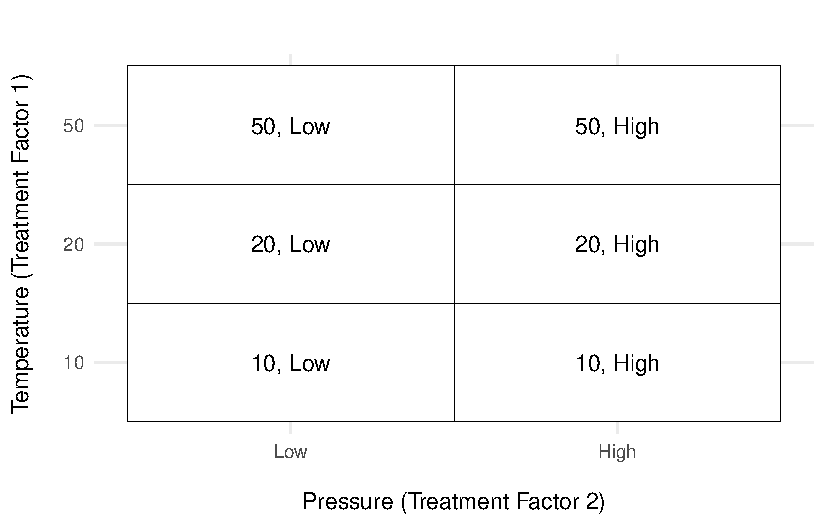
\includegraphics[keepaspectratio]{02_ExpDesign_Term_files/figure-pdf/fig-vistreat-1.pdf}}

}

\caption{\label{fig-vistreat}Visualization of how treatments are formed
as combinations of treatment levels.}

\end{figure}%

In the figure above, there are two treatment factors: Temperature (on
the y-axis) and Pressure (on the x-axis). The axis ticks represent the
levels of each treatment factor, and the blocks within the grid
represent the treatments, which are specific combinations of the levels
of Temperature and Pressure. Each treatment is labeled with the
corresponding combination of levels (e.g., `50, Low' or `10, High').

\begin{tcolorbox}[enhanced jigsaw, coltitle=black, title={Example 1}, breakable, bottomtitle=1mm, bottomrule=.15mm, colback=white, toprule=.15mm, rightrule=.15mm, opacitybacktitle=0.6, arc=.35mm, toptitle=1mm, colframe=quarto-callout-warning-color-frame, colbacktitle=quarto-callout-warning-color!10!white, titlerule=0mm, leftrule=.75mm, opacityback=0, left=2mm]

Three groups of students, 5 in each group, were receiving therapy for
severe test anxiety. Group 1 received 5 hours, group 2 received 10 hours
and group 3 received 15 hours. At the end of therapy each subject
completed an evaluation of test anxiety. Did the amount of therapy have
an effect on the level of test anxiety?

The three groups of students received the scores on the Test Anxiety
index (TAI) at the end of treatment shown in the table below.

\begin{longtable}[]{@{}ccc@{}}
\toprule\noalign{}
Group 1 & Group 2 & Group 3 \\
\midrule\noalign{}
\endhead
\bottomrule\noalign{}
\endlastfoot
48 & 55 & 51 \\
50 & 52 & 52 \\
53 & 53 & 50 \\
52 & 55 & 53 \\
50 & 53 & 50 \\
\end{longtable}

\hfill\break

\end{tcolorbox}

When faced with a text like this, it is useful to identify the treatment
factors, their levels and the treatments, as well the response. Clearly,
from the question, we are interested in the effect of therapy on test
anxiety. A statement like this can generally be read as the effect of
the treatment factor on the response. Nowhere is another treatment
factor mentioned, so we only have one in this example. What are the
levels of therapy we set? The levels are 5, 10 and 15 hours of therapy
and since we only have one factor these are also the treatments. Let's
summarise this as follows:

\begin{itemize}
\tightlist
\item
  \textbf{Response:} Test Anxiety\\
\item
  \textbf{Treatment Factor:} Therapy\\
\item
  \textbf{Treatment Levels:} 5, 10, and 15 hours of therapy\\
\item
  \textbf{Treatments:} 5, 10, and 15
\end{itemize}

\section*{\texorpdfstring{\textbf{Experimental and observational
unit}}{Experimental and observational unit}}\label{experimental-and-observational-unit}
\addcontentsline{toc}{section}{\textbf{Experimental and observational
unit}}

\markright{\textbf{Experimental and observational unit}}

The \textbf{experimental unit} is the entity (e.g.~material, object, or
individual) to which a treatment is assigned or that receives the
treatment. By contrast, the \textbf{observational unit} is the entity
from which the response is recorded. This distinction is very important
because it is the experimental units which determine how often the
treatment has been replicated and therefore the precision with which we
can measure the treatment effect. In the methods that we cover in this
course, we require that in the end there is only one `observation'
(response value) per experimental unit. If several measurements have
been taken on an experimental unit, we will combine these into one
observation, typically by taking the mean. Very often, the experimental
unit is also the observational unit.

What are the experimental units? To determine this, revisit the text of
Example 1 and ask yourself: what entity received the treatments or to
what were treatments applied? Most of you, will probably answer the
students and this is correct. Each student received the respective
treatment (number of hours in therapy) assigned to their group and so
there are \(5 \times 3 = 15\) experimental units.

There is an argument to be made that it is not clear whether the
students received therapy on their own or that the groups of students
received therapy together. In that case, treatments were applied to
groups of students and so there would be three experimental units. This
will usually be clear from the text, but we'll use this scenario to
illustrate some concepts as we go.

We also need to know what the observational units are. The text states
that at the end of therapy, each student completed an evaluation to
determine their level of test anxiety. So the response, test anxiety,
was measured on the student level which means students are the
observational units. In the first scenario, the students are both the
experimental units and observational units. But this would not be the
case if groups are the experimental unit.

We also require that there is only one observation per experimental
unit, the first scenario meets this requirement. For the second
scenario, we have 5 observations per group and so we would have to take
the mean of these values to end up with one response value per group.

Let's add to the summary assuming students are the experimental units:

\begin{itemize}
\tightlist
\item
  \textbf{Experimental unit (no):} Student (15)\\
\item
  \textbf{Observational unit (no):} Student (15)
\end{itemize}

\section*{\texorpdfstring{\textbf{Homogeneity of experimental
units}}{Homogeneity of experimental units}}\label{homogeneity-of-experimental-units}
\addcontentsline{toc}{section}{\textbf{Homogeneity of experimental
units}}

\markright{\textbf{Homogeneity of experimental units}}

When the set of experimental units are as similar as possible such that
there are no distinguishable differences between them, they are said to
be \textbf{homogeneous} (a fancy word for saying they are of the same
kind). The more homogeneous the units are, the smaller the experimental
error variance (natural variation between between observations of the
same treatments) will be. It is super important to have fairly
homogeneous units because it allows us to detect differences between
treatments more easily.

\section*{\texorpdfstring{\textbf{Blocking}}{Blocking}}\label{blocking}
\addcontentsline{toc}{section}{\textbf{Blocking}}

\markright{\textbf{Blocking}}

If the experimental units are not fairly similar but are heterogeneous
(the opposite of homogeneous), we can group them into sets of similar
units. This process is called \textbf{blocking} and the groups are
considered ``blocks''. We compare the treatments within each block as if
each block is its own mini-experiment. This way we account for the
differences between blocks and can better isolate the effect of the
treatments.

\begin{tcolorbox}[enhanced jigsaw, coltitle=black, title={Example 2}, breakable, bottomtitle=1mm, bottomrule=.15mm, colback=white, toprule=.15mm, rightrule=.15mm, opacitybacktitle=0.6, arc=.35mm, toptitle=1mm, colframe=quarto-callout-warning-color-frame, colbacktitle=quarto-callout-warning-color!10!white, titlerule=0mm, leftrule=.75mm, opacityback=0, left=2mm]

Imagine you're testing the effectiveness of two marketing strategies (A
and B) to increase sales at a chain of coffee shops. The coffee shops
are located in different neighborhoods, where factors like income levels
might influence sales. To prevent these differences from skewing the
results, you group the coffee shops into ``blocks'' based on
neighborhood characteristics such as income level (e.g., low, medium,
high).

Within each block, you randomly assign coffee shops to either Strategy A
or Strategy B. This approach allows you to compare the strategies while
controlling for variability caused by differences in neighborhood
features.

Without blocking, would you be able to confidently attribute differences
in sales to the strategies alone? Likely not, as any observed
differences could be due to neighborhood-specific factors rather than
the strategies themselves.

\end{tcolorbox}

\section*{\texorpdfstring{\textbf{Replication and
pseudoreplication}}{Replication and pseudoreplication}}\label{replication-and-pseudoreplication}
\addcontentsline{toc}{section}{\textbf{Replication and
pseudoreplication}}

\markright{\textbf{Replication and pseudoreplication}}

If a treatment is applied independently to more than one experimental
unit it is said to be \textbf{replicated}. Treatments must be
replicated! Making more than one observation on the same experimental
unit is not replication, but \emph{pseudoreplication}. Pseudoreplication
is a common fallacy. The problem is that without true replication, we
don't have an estimate of uncertainty, of how repeatable, or how
variable the result is if the same treatment were to be applied
repeatedly.

In Example 1, if experimental units were the groups and we didn't take
the average of the observations per group, we would have
pseudoreplication as each student would not be an independent replicate
of a treatment - effectively, we have only applied each treatment once.
You might notice that we then only have one true replicate per treatment
group and this is problematic. To get an estimate of uncertainty, we
would have to repeat this experiment a few more times to get more than
one proper replicate.

The first scenario, however, did not have this problem and each
treatment was replicated five times. After going through all this, we
have the following summary:

\begin{itemize}
\tightlist
\item
  \textbf{Response:} Test Anxiety\\
\item
  \textbf{Treatment Factor:} Therapy\\
\item
  \textbf{Treatment Levels:} 5, 10, and 15 hours of therapy\\
\item
  \textbf{Treatments:} 5, 10, and 15\\
\item
  \textbf{Experimental unit (no):} Student (15)\\
\item
  \textbf{Observational unit (no):} Student (15)\\
\item
  \textbf{Replicates:} 5
\end{itemize}

\begin{tcolorbox}[enhanced jigsaw, coltitle=black, title=\textcolor{quarto-callout-tip-color}{\faLightbulb}\hspace{0.5em}{Tip}, breakable, bottomtitle=1mm, bottomrule=.15mm, colback=white, toprule=.15mm, rightrule=.15mm, opacitybacktitle=0.6, arc=.35mm, toptitle=1mm, colframe=quarto-callout-tip-color-frame, colbacktitle=quarto-callout-tip-color!10!white, titlerule=0mm, leftrule=.75mm, opacityback=0, left=2mm]

Creating a summary like this, is a handy exercise for any experiment you
come across, and we'll keep doing it for every experiment in this book.
As we go along, we'll also add information about the type of experiment
that was conducted.

\end{tcolorbox}

\chapter*{The three R's of experimental
design}\label{the-three-rs-of-experimental-design}
\addcontentsline{toc}{chapter}{The three R's of experimental design}

\markboth{The three R's of experimental design}{The three R's of
experimental design}

\textbf{Experimental Design} is a detailed procedure for grouping, if
blocking is necessary, experimental units and for how treatments are
assigned to the experimental units. There are three fundamental
principles, known as the `three R's of experimental design' which are at
the core of a good experiment. The following section might feel a bit
repetitive, but these concepts cannot be emphasised enough.

\section*{Replication}\label{replication}
\addcontentsline{toc}{section}{Replication}

\markright{Replication}

Let's define it again: replication is when each treatment is applied to
several experimental units. This ensures that the variation between two
or more units receiving the same treatment can be estimated and valid
comparisons can be made between treatments. In other words, replication
allows us to separate variation due to differences between treatments
from variation within treatments. For true replication, each treatment
should be \textbf{independently} applied to several experimental units.
If this is not the case, treatment effects become confounded with other
factors.

Confounding means that is not possible to separate the effects of two
(or more) factors on the response, i.e.~it is not possible to say which
of the two factors is responsible for any changes in the response. This
is what happened in the Example 1 when groups are the experimental
units. With only one replicate per treatment, the effect of therapy is
confounded with the experimental unit or the effect of group on test
anxiety. The reason why this is a problem is that any difference between
the treatments could be due to any differences between the groups and
not just the number of therapy hours. The same would be true if we only
had one student per group. Why? Take a moment to think about this.

Consider the first row of the data from Example 1. It looks like the
student in group 2 scored the highest, followed by group 3 and then
group 1. So does longer therapy sessions lead to higher test anxiety?
Likely not! With only one student per treatment, we are not able to say
that any differences in the response are due to the treatments. It could
be due to any differences between the individuals. Maybe the student in
group 3 tends to score higher on anxiety tests regardless of the
treatment, or perhaps the student in group 1 was unusually calm that
day. Without replication, these individual differences could mask (or
mimic) the true effects of the treatments.

By replicating the treatments across multiple students, we can average
out these individual differences and gain a clearer picture of whether
therapy duration truly impacts test anxiety. With five students per
group, we might observe that group 1 consistently scores lower than
group 3. This consistency would provide stronger evidence that the
treatments, and not just individual variation, are responsible for the
observed differences. So by replication, we can compare within treatment
variation to variation between treatments.

\begin{longtable}[]{@{}ccc@{}}
\toprule\noalign{}
Treatment 1 & Treatment 2 & Treatment 3 \\
\midrule\noalign{}
\endhead
\bottomrule\noalign{}
\endlastfoot
48 & 55 & 51 \\
50 & 52 & 52 \\
53 & 53 & 50 \\
52 & 55 & 53 \\
50 & 53 & 50 \\
\end{longtable}

\section*{Randomisation}\label{randomisation}
\addcontentsline{toc}{section}{Randomisation}

\markright{Randomisation}

Randomisation refers to the process of randomly assigning treatments to
experimental units such that each experimental unit has equal chance of
receiving a specific treatment. Randomisation ensures that:

\begin{enumerate}
\def\labelenumi{\arabic{enumi}.}
\item
  There is no bias on the part of the experimenter, either conscious or
  unconscious, when assigning treatments to experimental units.
\item
  No experimental unit is favored to receive a particular treatment.
\item
  Possible differences between units are equally distributed among
  treatments. If there are clear differences between units, then
  blocking should be performed and randomisation occurs within blocks.
  We'll talk more about this when we encounter Randomised Block Designs.
\item
  We can assume independence between observations.
\end{enumerate}

Randomisation is not haphazard. In statistics (and here in the context
of experimental design), randomisation has a specific meaning: namely
that each experimental unit has the same chance of being allocated any
of the treatments. This can be done using random number generators such
as with software packages, dice or drawing number from a hat (provided
the number have been shuffled adequately and have equal chance to be
picked).

Let's have a look at randomisation in R. Suppose we have 4 treatments
(\texttt{A}, \texttt{B}, \texttt{C}, and \texttt{D}) and 32 experimental
units. There are no differences between the units, so we don't have to
block, and we can equally split the units across the treatments, which
means we have 8 units per treatment, i.e., 8 replicates. In R, we first
create a long vector of 8 \texttt{A}s, 8 \texttt{B}s, 8 \texttt{C}s, and
8 \texttt{D}s called \texttt{all.treat}. Then shuffle the vector to
obtain a randomisation using the function \texttt{sample}.

\begin{Shaded}
\begin{Highlighting}[]
\CommentTok{\# repeat the vector A, B, C, D 8 times }
\NormalTok{all.treats }\OtherTok{\textless{}{-}} \FunctionTok{rep}\NormalTok{(}\FunctionTok{c}\NormalTok{(}\StringTok{"A"}\NormalTok{,}\StringTok{"B"}\NormalTok{,}\StringTok{"C"}\NormalTok{,}\StringTok{"D"}\NormalTok{), }\AttributeTok{times =} \DecValTok{8}\NormalTok{)}

\CommentTok{\# permutation of all.treats (sample withut replacement)}
\NormalTok{rand1 }\OtherTok{\textless{}{-}} \FunctionTok{sample}\NormalTok{(all.treats)}

\CommentTok{\# example output}
\NormalTok{rand1}
\end{Highlighting}
\end{Shaded}

\begin{verbatim}
 [1] "A" "C" "B" "D" "D" "D" "D" "D" "C" "B" "D" "A" "B" "A" "D" "C" "B" "C" "D"
[20] "C" "A" "A" "B" "A" "C" "A" "B" "C" "A" "B" "B" "C"
\end{verbatim}

Experimental unit 1 recipes the first treatment that appears as the
first element in the shuffled vector, experimental unit 2 receives the
second and so on.

\section*{Reduction of Unexplained Variation
(Blocking)}\label{reduction-of-unexplained-variation-blocking}
\addcontentsline{toc}{section}{Reduction of Unexplained Variation
(Blocking)}

\markright{Reduction of Unexplained Variation (Blocking)}

Unexplained variation (or experimental error variance or within
treatment variance) is largely due to inherent differences between
experimental units. The larger this unexplained variation, the more
difficult it becomes to detect treatment differences (a treatment
signal). To minimise experimental error variance we can control
extraneous factors (i.e.~keeping all else constant) and by choosing
homogeneous experimental units. Otherwise, we can block experimental
units to reduce the variation.

Blocking variables are nuisance factors that might affect your response
or introduce systematic variation in the response and we are typically,
not interested in these. Often, they are factors that cannot be
randomised, e.g.~biological sex of a person, time of day, location of a
warehouse etc. We control the effect of such variables on the response
by blocking for them so that we can investigate the possible effect of a
variable that we are interested in. Usually, in a complete block
experiment, there are as many experimental units per block as there are
treatments, so that each treatment is applied once in every block.
Treatments are randomized to the experimental units in the blocks. We
can then compare the effects of treatments on similar experimental
units, and we can estimate the variation induced in the response due to
the differences between blocks. This variation due to blocks can then be
removed from the unexplained variation.

Blocking also offers the opportunity to test treatments over a wider
range of conditions, e.g.~if I only use people of one age in my
experiment (say students) I cannot generalize my results to older
people. However, if i use different age blocks I will be able to tell
whether the treatments have similar effects in all age groups or not.

Lastly, if blocking is not feasible, randomization will ensure that at
least treatments and nuisance factors are not confounded.

\begin{quote}
``Block what you can, randomize what you cannot.''

--- Box, Hunter \& Hunter (1978)
\end{quote}

\chapter{Designing an Experiment}\label{designing-an-experiment}

When planning an experiment we need to decide on:

\begin{itemize}
\tightlist
\item
  treatment factors and their levels
\item
  the response
\item
  experimental material / units
\item
  blocking factors
\item
  number of replicates
\end{itemize}

Some of these will be determined by the research question and how
experimental units are assigned to treatments are determined by the
design. The design that will be chosen for a particular experiment
depends on the \textbf{treatment structure} (determined by the research
question) and the \textbf{blocking structure} (determined by the
available experimental units).

Here are two ways the treatments can be structured:

\begin{enumerate}
\def\labelenumi{\arabic{enumi}.}
\tightlist
\item
  \textbf{Single factor}: the treatments are the levels of a single
  treatment factor.
\item
  \textbf{Factorial}: when more than one factor are of interest, then
  the experiment is said to be a factorial experiment. The treatments
  are constructed by crossing the treatment factors like we did in
  Figure~\ref{fig-vistreat} such that the treatments are all possible
  combinations of the treatment levels. For example, if factor A has
  \(a\) levels and factor B has \(b\) levels, there are \(a \times b\)
  treatments. Such an experiment would then be called an \(a \times b\)
  factorial experiment.
\end{enumerate}

The blocking structure is determined the set of experimental units
chosen or available for the experiment.are there any
structures/differences that need to be blocked? Do I want to include
experimental units of different types to make the results more general?
How many experimental units are available in each block? For the
simplest design in this course, the number of experimental units in each
block corresponds to the number of treatments. This is called a complete
block experiment. There are several other blocking structures, such as
incomplete blocks and blocks with missing values, all with specific
analysis which we will not cover here.

In this course, we cover two basic designs: Completely Randomized
Designs (CRD) and Randomized Block Designs (RBD). For both designs, the
treatment structure can be single or factorial. Where they differ is in
terms of the experimental units and how randomization occurs.

\textbf{\emph{Completely Randomized Designs (CRD)}}

When all experimental units are fairly homogeneous, a CRD is used.
Treatments are randomized to all experimental units.

\textbf{\emph{Randomized Block Design}}

This design is used when all experimental units are not homogeneous or
blocking is required to control a nuisance factor. The treatments are
randomized to the units within blocks.

\part{Single Factor Completely Randomised Designs}

\chapter{Introduction}\label{introduction}

Completely Randomized Designs (CRDs) are the simplest experimental
designs. They are used when experimental units are uniform enough and we
expect them to react similar to a given treatment. In other words, we
have no reason to suspect that a group of experimental units might react
differently to the treatments. We also don't expect any effects (besides
possibly a treatment effect) to cause any systematic changes in the
response. So, we don't have to block for differing experimental units or
any nuisance factors.

Remember experimental design is the procedure for how experimental units
are grouped and treatments are applied. We have already said that there
are no blocks in CRDs. So randomisation occurs without restriction and
to all experimental units. More generally, each of the \(a\) treatments
are randomly assigned to \(r\) experimental units, such that each
experimental unit is equally likely to receive any of the treatments.
This means that there are \(N = r \times a\) experimental units in
total. We only consider designs that are \emph{balanced} meaning that
there an equal number of experimental units per treatment, i.e.~a
treatment is applied to \(r\) units. The experiment is then said to have
\(r\) replicates.

The aim when analysing CRDs is to determine whether there is an effect
of the treatment factor. We accomplish this by testing for differences
in the treatment means (mean of response values in each treatment)
through analyses different sources of variation in the response. This
will become clear as we progress.

\section{Example: The effect of social media multitasking on classroom
performance.}\label{example-the-effect-of-social-media-multitasking-on-classroom-performance.}

As a student, I used to believe I could multitask effectively. I would
scroll through my phone during lectures, study while texting friends, or
listen to podcast while driving. It felt like I was paying attention to
everything, but in hindsight, I can barely recall the details of those
podcasts. I often had to revisit lectures or restart study sessions
because my focus wasn't truly there. This tendency extends beyond
student life. In the average workplace, tasks are frequently interrupted
by social media, email checks, or notifications. Many of us feel the
constant pull of our phones when trying to concentrate, whether we're
working, studying, or even relaxing.

In an era of perceived multitasking, where devices and distractions
dominate our attention, it's worth asking: Does social media
multitasking impact academic performance of students?

\begin{tcolorbox}[enhanced jigsaw, coltitle=black, title={Example 5.1}, breakable, bottomtitle=1mm, bottomrule=.15mm, colback=white, toprule=.15mm, rightrule=.15mm, opacitybacktitle=0.6, arc=.35mm, toptitle=1mm, colframe=quarto-callout-warning-color-frame, colbacktitle=quarto-callout-warning-color!10!white, titlerule=0mm, leftrule=.75mm, opacityback=0, left=2mm]

Two researchers from Turkey, Demirbilek and Talan (2018), conducted a
study to try and answer this question. Specifically, they examined the
impact of social media multitasking during live lectures on students'
academic performance.

A total of 120 first-year undergraduate students from the same Turkish
University were randomly assigned to one of three groups:

\begin{enumerate}
\def\labelenumi{\arabic{enumi}.}
\tightlist
\item
  \textbf{Control Group:} Students used traditional pen-and-paper
  note-taking.
\item
  \textbf{Experimental Group 1 (Exp 1):} Students engaged in SMS texting
  during the lecture.
\item
  \textbf{Experimental Group 2 (Exp 2):} Students used Facebook during
  the lecture.
\end{enumerate}

Over a three-week period, participants attended the same lectures on
Microsoft Excel. To measure academic performance, a standardised test
was administered.

\end{tcolorbox}

\textbf{The analysis of experimental data is determined by the design.}
This is the first thing we need to investigate. The design dictates the
terms that we will include in our statistical model and so it is crucial
to be able to identify the design and all factors included (blocking and
treatment). It is also important to check that randomisation has been
done correctly and determine the number of replicates used. In the
previous chapter we started doing this by creating a summary of the
design and we do the same here. From the description of the study, it is
clear that:

\begin{itemize}
\tightlist
\item
  \textbf{Response Variable:} Academic performance, as measured by test
  scores.
\item
  \textbf{Treatment Factor:} Level of social media multitasking.
\item
  \textbf{Treatment Levels (Groups):} Control, Exp 1, and Exp 2.
\end{itemize}

Students were randomly assigned to one of the three groups, and
performance was measured for each individual. Although this may seem
obvious, they only took one measurement per student, so we don't have to
worry about pseudoreplication. This setup indicates that the students
are both the experimental units and the observational units in this
study. With a total of 120 experimental units and three treatments, the
experiment has 40 replicates. Since only one treatment factor was
investigated, and no blocking was performed, this is classified as a
\textbf{single-factor Completely Randomized Design (CRD).} Here is the
study breakdown:

\begin{itemize}
\tightlist
\item
  \textbf{Response Variable:} Academic Performance\\
\item
  \textbf{Treatment Factor:} Level of Social Media Multitasking\\
\item
  \textbf{Treatment Levels:} Control, Experimental 1 (SMS), Experimental
  2 (Facebook)\\
\item
  \textbf{Treatments:} Control, Experiment 1, Experiment 2\\
\item
  \textbf{Experimental Unit:} Student (120)\\
\item
  \textbf{Observational Unit:} Student (120)\\
\item
  \textbf{Replicates:} 40 students per group\\
\item
  \textbf{Design Type:} Single-Factor Completely Randomized Design (CRD)
\end{itemize}

Before we continue, now is the time to note that we won't be using the
real data collected in this experiment. It wasn't available but I have
simulated data to match their results. I've also made some other
modifications such as the original study included 122 students but to
ensure a balanced design I include only 120.

\section{Exploratory data analysis
(EDA)}\label{exploratory-data-analysis-eda}

Before we start any analyses, we have to conduct some exploratory data
analysis to get a feel for our data. We start by checking whether it has
been read in correctly and then look at some descriptive statistics.

In R, we read in the data set and then use some commands to inspect the
data set:

\begin{Shaded}
\begin{Highlighting}[]
\NormalTok{multitask }\OtherTok{\textless{}{-}} \FunctionTok{read.csv}\NormalTok{(}\StringTok{"Datasets/multitask\_performance.csv"}\NormalTok{)}
\FunctionTok{nrow}\NormalTok{(multitask) }\CommentTok{\# check number of rows}
\end{Highlighting}
\end{Shaded}

\begin{verbatim}
[1] 120
\end{verbatim}

\begin{Shaded}
\begin{Highlighting}[]
\FunctionTok{head}\NormalTok{(multitask) }\CommentTok{\# check first 5 rows }
\end{Highlighting}
\end{Shaded}

\begin{verbatim}
    Group Posttest
1    Exp1 86.39427
2    Exp1 64.19996
3    Exp2 52.75394
4 Control 67.81147
5    Exp1 52.39911
6    Exp1 56.58150
\end{verbatim}

\begin{Shaded}
\begin{Highlighting}[]
\FunctionTok{tail}\NormalTok{(multitask) }\CommentTok{\# check last 5 rows }
\end{Highlighting}
\end{Shaded}

\begin{verbatim}
      Group Posttest
115 Control 77.94344
116 Control 63.58444
117    Exp1 55.17758
118    Exp2 67.16150
119    Exp2 32.58373
120    Exp2 49.58119
\end{verbatim}

\begin{Shaded}
\begin{Highlighting}[]
\FunctionTok{summary}\NormalTok{(multitask)}
\end{Highlighting}
\end{Shaded}

\begin{verbatim}
    Group              Posttest    
 Length:120         Min.   :23.38  
 Class :character   1st Qu.:52.67  
 Mode  :character   Median :65.01  
                    Mean   :63.59  
                    3rd Qu.:76.32  
                    Max.   :98.78  
\end{verbatim}

The data set consists of 120 rows (each row representing a student) and
two columns (\texttt{Group} and \texttt{Posttest}). The first column,
\texttt{Groups}, contains the treatment the student was assigned and the
\texttt{Posttest} column contains the response measure. Using the
functions \texttt{head} and \texttt{tail}, we can look at the first and
last 5 rows and the function \texttt{summary} provides us with a
description of each column. We do this to check that R has read in our
data correctly (you can view the whole data set by running
\texttt{view(multitask)} as well). The summary tells us that the
\texttt{Group} column is of the class ``character''. For our analysis,
we want it to be read as a factor:

\begin{Shaded}
\begin{Highlighting}[]
\NormalTok{multitask}\SpecialCharTok{$}\NormalTok{Group }\OtherTok{\textless{}{-}} \FunctionTok{as.factor}\NormalTok{(multitask}\SpecialCharTok{$}\NormalTok{Group)}
\FunctionTok{summary}\NormalTok{(multitask)}
\end{Highlighting}
\end{Shaded}

\begin{verbatim}
     Group       Posttest    
 Control:40   Min.   :23.38  
 Exp1   :40   1st Qu.:52.67  
 Exp2   :40   Median :65.01  
              Mean   :63.59  
              3rd Qu.:76.32  
              Max.   :98.78  
\end{verbatim}

Now, we can see that there are 40 replicates per treatment group,
confirming that the experiment is balanced. I have assumed that, based
on the results shown, that the \texttt{Posttest} scores were recorded as
percentages and using the summary we can quickly check whether there are
any observations that are not on the appropriate scale or might be
outliers. Looks good so far!

\section{Checking assumptions}\label{checking-assumptions}

Demirbilek and Talan (2018) had several research questions, but here we
only consider the following:

Are there any differences in mean academic performance between the three
groups?

You might think that we could perform three t-tests (Control vs Exp 1,
Control vs Exp 3, Exp 1 vs Exp 2). We could, but the problem with this
approach is what we call multiple testing. When conducting many tests,
there is an increased risk of making a Type 1 Error (rejecting the null
hypothesis when it is in fact true) \footnote{Can't remember what a
  \(t\)-test is and/or need a refresher on hypothesis testing? Have a
  look this video on t-tests and document for a brief reminder.
  \textbf{Also, a quick (and cool) sidenote:} This study by Chen et al.
  (2024) used a Completely Randomized Design (CRD), randomly assigning
  undergraduate students to playback speed groups (1x, 1.5x, 2x, and
  2.5x) to measure the effect on comprehension of recorded lectures.
  Using ANOVA they found that comprehension was preserved up to 2x
  speed. I personally like to increase the playback speed to 1.5px if I
  just need to revise something quickly.}.

When we have more than two groups, we can use a one-way analysis of
variance (ANOVA) which can be seen as an extension of a \(t\)-test and
is called ``one-way'' because there is a single factor being considered.
In the next section, we will see that ANOVA is a linear model and some
of the assumptions are about the model errors (just like regression):

\begin{enumerate}
\def\labelenumi{\arabic{enumi}.}
\tightlist
\item
  There are no outliers.
\item
  The errors are independent.
\item
  The errors are normally distributed.
\item
  All groups have equal population variances.
\end{enumerate}

We need to check the validity of these assumptions. There are both
formal and informal techniques. Formal techniques (i.e.~hypothesis
tests) are not always appropriate for several reasons such as small data
sets or that testing one assumption usually requires that the other two
hold, complicating the order of tests. Informal techniques are more than
sufficient and in this course, we stick with them.

\subsection*{Outliers}\label{outliers}
\addcontentsline{toc}{subsection}{Outliers}

Outliers are unusual observations (response values) that deviate
substantially from the remaining data points. They can have a large
influence on the estimates of our model. Think of statistics such as
means and variances, outlying observations will shift the mean towards
them and distort the variability of the data.

If we're lucky, outliers are artefacts of data recording or entering
issues, such as a missing decimal points or incorrect scaling (called
error outliers). These types of outliers can be corrected and the
analysis can be done as usual. If, however, there are freak observations
that are not clearly due to anything like data inputting, then they are
likely genuine unusual responses (called interesting outliers) and
should not be discarded. There are many ways of identifying and dealing
with outliers (Aguinis, Gottfredson, and Joo (2013) found 29 different
ways in the literature). Here, it is recommended that the analysis
should be run with and without the outliers to see whether the
conclusion depends on their inclusion. When dealing with outliers, it is
best to be transparent and clear about how they were handled. Simply
removing outliers with no explanation is questionable research practice.

A good way to check for outliers, is to inspect the data visually with a
box-plot of your data grouped by treatment.

\begin{Shaded}
\begin{Highlighting}[]
\FunctionTok{boxplot}\NormalTok{(Posttest }\SpecialCharTok{\textasciitilde{}}\NormalTok{ Group, }\AttributeTok{data =}\NormalTok{ multitask, }\AttributeTok{col =} \FunctionTok{c}\NormalTok{(}\StringTok{"skyblue"}\NormalTok{, }\StringTok{"lightgreen"}\NormalTok{, }\StringTok{"pink"}\NormalTok{), }
        \AttributeTok{main =} \StringTok{"Posttest Scores by Group"}\NormalTok{, }
        \AttributeTok{xlab =} \StringTok{"Group"}\NormalTok{, }
        \AttributeTok{ylab =} \StringTok{"Posttest Scores"}\NormalTok{)}

\FunctionTok{stripchart}\NormalTok{(Posttest}\SpecialCharTok{\textasciitilde{}}\NormalTok{Group, }\AttributeTok{data =}\NormalTok{ multitask, }\AttributeTok{vertical =} \ConstantTok{TRUE}\NormalTok{, }\AttributeTok{add =} \ConstantTok{TRUE}\NormalTok{, }\AttributeTok{method =} \StringTok{"jitter"}\NormalTok{)}
\end{Highlighting}
\end{Shaded}

\begin{figure}[H]

\centering{

\pandocbounded{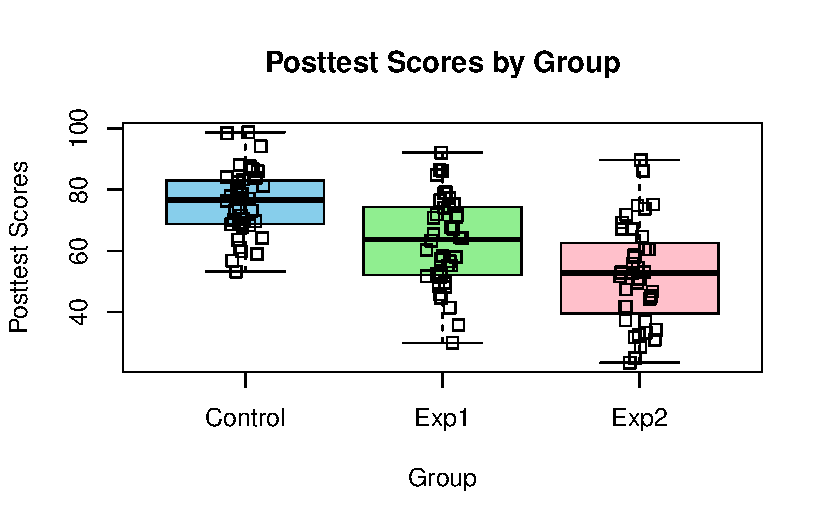
\includegraphics[keepaspectratio]{05_CRD_Intro_files/figure-pdf/fig-socialbox-plot-1.pdf}}

}

\caption{\label{fig-socialbox-plot}Box-plots of Post treatment scores by
group.}

\end{figure}%

The first line of code plots the box-plot and by inputting
\texttt{Posttest\textasciitilde{}Groups} as the first argument we are
say plot the values of \texttt{Posttest} by \texttt{Groups}. There are
extra graphical parameters specified to make the plot look a bit nicer.
The function \texttt{stripchart} is used to overlay the data points.
Based on these plots, there aren't any obvious outlying observations.

\subsection*{Equal population variance}\label{equal-population-variance}
\addcontentsline{toc}{subsection}{Equal population variance}

The model assumes that population variances in different levels of the
treatment factor are equal. That is, it is assumed in ANOVA that the
variance of the response within each treatment is a separate estimate of
the same population variance.

Since we only have sample data, we would not expect that the sample
variances to be exactly the same. If they are different it does not mean
the assumption is not met. We expect them to differ a bit due to chance
simply because we are sampling. Every time we sample from a population,
the data set will be different and so will it's variability. The sample
variances need to be similar enough so that our assumption of equal
population variance is reasonable.

To check this assumption, we can inspect the box-plots again and compare
the heights. More specifically, we look at the interquartile ranges
(IQR). From looking at the plot, the IQRs do not vary widely. If you
prefer to look at the actual values, we can use R to obtain them:

\begin{Shaded}
\begin{Highlighting}[]
\FunctionTok{sort}\NormalTok{(}\FunctionTok{tapply}\NormalTok{(multitask}\SpecialCharTok{$}\NormalTok{Posttest,multitask}\SpecialCharTok{$}\NormalTok{Group,IQR))}
\end{Highlighting}
\end{Shaded}

\begin{verbatim}
 Control     Exp2     Exp1 
14.01068 20.94529 21.97001 
\end{verbatim}

Another measure of variability we can look at, are the standard
deviations (sd's). With the same line of code but just replacing the
function we want to apply, we obtain the sd of each group:

\begin{Shaded}
\begin{Highlighting}[]
\FunctionTok{sort}\NormalTok{(}\FunctionTok{tapply}\NormalTok{(multitask}\SpecialCharTok{$}\NormalTok{Posttest,multitask}\SpecialCharTok{$}\NormalTok{Group,sd))}
\end{Highlighting}
\end{Shaded}

\begin{verbatim}
 Control     Exp1     Exp2 
10.82887 14.60601 16.42678 
\end{verbatim}

The rule of thumb is to use the ratio of the smallest to largest
standard deviation and check whether it is smaller than five. In our
case, the smallest sd (of the Control group) is about 1.5 times smaller
than the largest sd (of the Exp 2 group) which is acceptable.

\subsection*{Normally distributed
errors}\label{normally-distributed-errors}
\addcontentsline{toc}{subsection}{Normally distributed errors}

We can check this assumption by looking at the residuals after model
fitting. A common misconception is to think that the response needs to
be normally distributed. However, it is only the unexplained variation,
i.e.~the errors or residuals (estimates of errors), that we assume to be
normally distributed. Of course, if the response has a clearly
non-normal distribution (e.g.~Binomial), then the residuals are likely
to be non-normal as well. So, we can check our response values before
hand for obvious deviation from normality, but we have to check this
assumption again after fitting our model. Things to look for are
asymmetric box-plots which indicate skew distributions. We also want to
check that the data points tend to cluster around the median. In
Figure~\ref{fig-socialbox-plot}, there are no signs of any clear
deviation from normality. Other graphs we could look at are histograms
or Quantile-Quantile (Q-Q) plots. Q-Q plots show the theoretical
quantiles of the standard normal distribution against the actual
quantiles of our data. We want our data to be as close to the xy line as
possible (deviations in the tails are expected).

\begin{Shaded}
\begin{Highlighting}[]
\FunctionTok{par}\NormalTok{(}\AttributeTok{mfrow =} \FunctionTok{c}\NormalTok{(}\DecValTok{1}\NormalTok{,}\DecValTok{3}\NormalTok{))}

\CommentTok{\# First we subset the data for each group}
\NormalTok{control }\OtherTok{\textless{}{-}}\NormalTok{ multitask}\SpecialCharTok{$}\NormalTok{Posttest[multitask}\SpecialCharTok{$}\NormalTok{Group }\SpecialCharTok{==} \StringTok{"Control"}\NormalTok{]}
\NormalTok{exp1 }\OtherTok{\textless{}{-}}\NormalTok{ multitask}\SpecialCharTok{$}\NormalTok{Posttest[multitask}\SpecialCharTok{$}\NormalTok{Group }\SpecialCharTok{==} \StringTok{"Exp1"}\NormalTok{]}
\NormalTok{exp2 }\OtherTok{\textless{}{-}}\NormalTok{ multitask}\SpecialCharTok{$}\NormalTok{Posttest[multitask}\SpecialCharTok{$}\NormalTok{Group }\SpecialCharTok{==} \StringTok{"Exp2"}\NormalTok{]}


\FunctionTok{qqnorm}\NormalTok{(control, }\AttributeTok{pty =} \DecValTok{4}\NormalTok{, }\AttributeTok{col =}\StringTok{"blue"}\NormalTok{, }\AttributeTok{main =} \StringTok{"Control"}\NormalTok{)}
\FunctionTok{qqline}\NormalTok{(control, }\AttributeTok{col =} \StringTok{"red"}\NormalTok{)}

\FunctionTok{qqnorm}\NormalTok{(exp1, }\AttributeTok{pty =} \DecValTok{4}\NormalTok{, }\AttributeTok{col =}\StringTok{"blue"}\NormalTok{, }\AttributeTok{main =} \StringTok{"Exp 1"}\NormalTok{)}
\FunctionTok{qqline}\NormalTok{(exp1, }\AttributeTok{col =} \StringTok{"red"}\NormalTok{)}

\FunctionTok{qqnorm}\NormalTok{(exp2, }\AttributeTok{pty =} \DecValTok{4}\NormalTok{, }\AttributeTok{col =}\StringTok{"blue"}\NormalTok{, }\AttributeTok{main =} \StringTok{"Exp 2"}\NormalTok{)}
\FunctionTok{qqline}\NormalTok{(exp2, }\AttributeTok{col =} \StringTok{"red"}\NormalTok{)}
\end{Highlighting}
\end{Shaded}

\begin{figure}[H]

\centering{

\pandocbounded{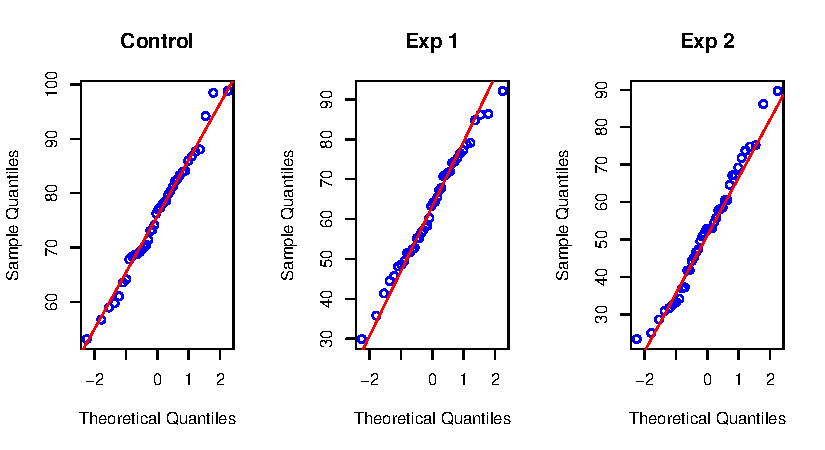
\includegraphics[keepaspectratio]{05_CRD_Intro_files/figure-pdf/fig-socialqq-1.pdf}}

}

\caption{\label{fig-socialqq}Q-Q plots of response per treatment group.}

\end{figure}%

The \texttt{qqnorm} function plots the theoretical quantiles on the
x-axis and the sample quantile son the y-axis. So each point on the plot
corresponds to a quantile from the sample plotted against the expected
quantile from the standard normal distribution. As a reference we add a
straight 45-degree line (in red) using the \texttt{qqline} function to
indicate what perfect normality would look like.

\subsection*{Independent errors}\label{independent-errors}
\addcontentsline{toc}{subsection}{Independent errors}

The assumption is that the \textbf{errors} are independent. While we can
check for certain types of dependence in the residuals after fitting the
ANOVA (as we will see later), dependence among observations generally
results in dependent residuals. Therefore, before fitting any models, we
examine the observations and the experimental design to identify
potential violations of independence.

In statistics, if one observation influences another in some way or
another, they are said to be dependent. For the type of data considered
here, there are two types of independence we require. Firstly,
observations within treatments should be independent and second,
observations between samples should be independent. Another way of
saying this, is \textbf{there should be independence within and among
treatments.} Depending on the direction of any violations, the within
treatment variance or among treatment variance can either be deflated or
inflated and treatment effects can be biased. This has considerable
impact on the test statistic (F-ratio for ANOVA, more on this later)
which could lead to misleading results. \footnote{Underwood (1996) has a
  very detailed explanation of the independence assumption (and the
  others) in the context of ANOVA. The book is for ecological
  experiments, but much of it pertains to all types of experiments.}

Violations of independence typically occur when the experimental units
within or among treatments are connected in some way. Dependence within
a sample can occurs when they are taken in a non-random sequence. Doing
so typically allows some other variable to introduce dependence between
successive observations. For example, measurement drift (when a tool's
reading gradually changes over time), physical effects
(e.g.~temperature) of the location of experimental units or the
experimenter might become better (or worse) at taking the measurement as
they move along. If these variables are not taken into account (by
including them as factors in the model), it leads to a lack of
independence in the errors of our model. Specifically, they lead to
auto-correlated residuals; observations made closer together in time or
space are more similar to each other than expected (this is what we
check after model fitting).

An informal check we could do, is to plot the data in the order in which
they were collected (if this information is available) whether that is
temporally or spatially to see if any patterns emerge. To do this in R,
we can create a Cleveland dot plot.

\begin{Shaded}
\begin{Highlighting}[]
\FunctionTok{dotchart}\NormalTok{(multitask}\SpecialCharTok{$}\NormalTok{Posttest, }\AttributeTok{ylab =} \StringTok{"Order of observation"}\NormalTok{, }\AttributeTok{xlab =}\StringTok{"Post treatment test score"}\NormalTok{)}
\end{Highlighting}
\end{Shaded}

\begin{figure}[H]

\centering{

\pandocbounded{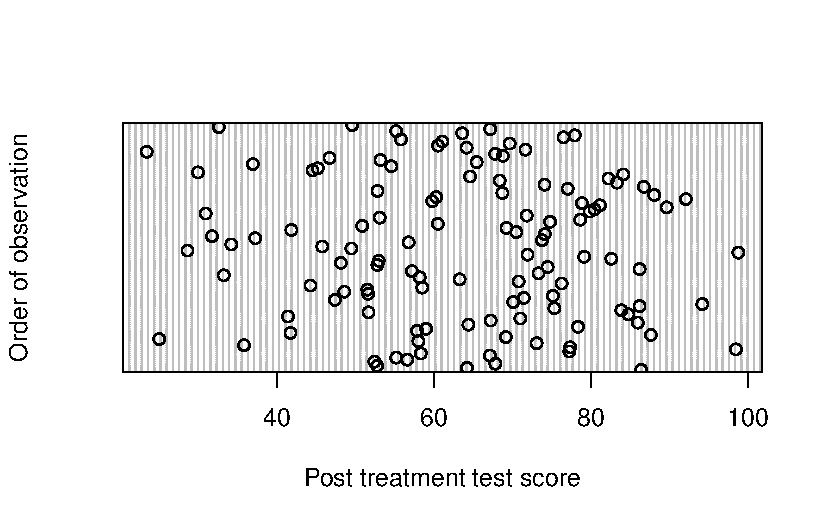
\includegraphics[keepaspectratio]{05_CRD_Intro_files/figure-pdf/fig-socialdotchart-1.pdf}}

}

\caption{\label{fig-socialdotchart}Cleveland dot chart of response
values in the order in which they appear in the data set.}

\end{figure}%

We have assumed that the order in which the observations appear in the
data set are the order in which they were recorded. If there were any
factors that caused systematic trends, (i.e.~dependence) in the
observations, then there would be some kind of pattern in the dot chart.
For our example, there is no clear pattern. After fitting the model, we
can also plot the residuals against spatial coordinate or against order
to check for obvious patterns. This method, however, only detects
violations of independence if observations are related to time or space.

Dependence between treatments can occur if we apply the treatments to
the same group of experimental units or if experimental units from
different treatments are able to interact in some way during the
experiment. These types of violations including those mentioned above,
are ones that we can mostly prevent or control by properly designing the
experiment. When we control for factors that might induce dependence, we
can include them in our model.

Other reasons for dependence may not be as obvious or easy to eliminate
as we will see below. In the end, they may not have a strong impact on
our estimates but it is important to carefully scrutinize your design
and the system you are studying to identify possible sources of
dependence so that these can be addressed and dealt with properly.

In our example, within and among group dependence could be caused by the
students interacting or influencing each other in some way (by sharing
notes for example). During the lectures, this can be controlled by
careful monitoring and randomising their position in the lecture
theater, but outside of lectures, it is less easy to control. Here we
can argue that if students interacted outside of lectures the impact on
their academic performance (as measured by the test) would likely be
negligible. The integrity of the students is at play. It is not really
possible to diagnose this type of dependence after the fact, only with
careful design and implementation can these be avoided.

\textbf{It is the onus of the experimenter to design and conduct
experiments that ensure independence.} With more thought (and if we're
lucky, funding) all well-designed experiments should lead to independent
data. If violations are found after the fact, they cannot typically be
corrected and then methods that deal specifically with dependent data
(if appropriate) should be used\footnote{A few of these methods are
  repeated measures ANOVA, mixed-models or hierarchical models.}.

\subsection*{A quick note on the robustness of
ANOVA}\label{a-quick-note-on-the-robustness-of-anova}
\addcontentsline{toc}{subsection}{A quick note on the robustness of
ANOVA}

A statistical procedure is said to be robust to departures from a model
assumption if the results remain unbiased even when the assumption is
not met. The robustness of ANOVA is as follows:

\begin{enumerate}
\def\labelenumi{\arabic{enumi}.}
\item
  The assumption of normality is not super crucial. Only severe
  departures from normality such as long-tailed distributions or skewed
  distributions when sample sizes are unequal and/or small are
  particularly problematic.
\item
  Independence within and among groups is extremely important. ANOVA
  does not handle dependent data and other analyses should be attempted
  if there is dependence.
\item
  ANOVA is relatively robust to violations of the equal variance
  assumption as long as there are no outliers, sample sizes are large
  and fairly equal (in the case of unbalanced designs which we do not
  cover here), and the sample variances are relatively equal.
\item
  ANOVA is not very resistant to severely outlying observations either.
\end{enumerate}

\begin{tcolorbox}[enhanced jigsaw, coltitle=black, title=\textcolor{quarto-callout-tip-color}{\faLightbulb}\hspace{0.5em}{Note}, breakable, bottomtitle=1mm, bottomrule=.15mm, colback=white, toprule=.15mm, rightrule=.15mm, opacitybacktitle=0.6, arc=.35mm, toptitle=1mm, colframe=quarto-callout-tip-color-frame, colbacktitle=quarto-callout-tip-color!10!white, titlerule=0mm, leftrule=.75mm, opacityback=0, left=2mm]

\begin{enumerate}
\def\labelenumi{\arabic{enumi}.}
\item
  In this course, you will always encounter data that has already been
  collected and the description of the experiment will likely not be
  very exhaustive. You might be task then with thinking about how the
  assumption of independence could have been violated, but for the most
  part we will assume the data are independent, both within and among
  samples (unless otherwise stated or you are asked if the assumption
  holds).
\item
  No real data set ever meets all assumptions of a model perfectly. As
  the famous (at least in the world of statistics) quote by George Box
  goes: ``All models are wrong but some are useful.'' Judging whether a
  particular data set meets our assumptions reasonably well is therefore
  a bit of an art. You will likely read and hear that being able to
  identify violations comes from \textbf{experience}. The best way to
  get experience is to look at lots of data sets where you know how well
  they meet the assumptions. That's best done via simulation. We
  therefore encourage you to use the attached R code to simulate data
  where various assumptions are violated. Run the code a number of times
  to get a feeling for how variable your actual sample can be even if
  the data generating mechanism doesn't change. You may also want to
  play around with the sample sizes and you can change the degree to
  which the assumptions are violated to get a feeling for how these
  violations show up in the plots.
\end{enumerate}

\end{tcolorbox}

\section{Summary}\label{summary}

Completely Randomized Designs (\textbf{CRDs}) are the simplest
experimental designs, used when experimental units are \textbf{uniform}
and expected to react similarly to treatments. Since no nuisance factors
are controlled, randomization occurs \textbf{without restriction}, and
treatments are \textbf{evenly assigned} across experimental units
(\textbf{balanced design}).

The social media multitasking study served as an example, where 120
students were randomly assigned to three groups (Control, SMS, Facebook)
to measure their academic performance. This setup represents a
single-factor CRD, where students are both the experimental and
observational units with 40 replicates per group.

Before conducting ANOVA, we:

\begin{itemize}
\tightlist
\item
  Checked the data set for correct structure (120 observations,
  treatment groups as factors).
\item
  Inspected summary statistics and visualized distributions (box-plots,
  histograms, Q-Q plots).
\end{itemize}

For ANOVA, the following assumptions were examined:

\begin{enumerate}
\def\labelenumi{\arabic{enumi}.}
\tightlist
\item
  \textbf{Outliers}: Check via box-plots.
\item
  \textbf{Equal variance}: Assess using interquartile ranges and ratio
  of sample standard deviations.
\item
  \textbf{Normality of errors}: Verified using Q-Q plots.
\item
  \textbf{Independence within and between treatment groups}: Considered
  through study design.
\end{enumerate}

Proper experimental design ensures valid conclusions. Identifying
violations of assumptions early helps prevent biased results.

\phantomsection\label{refs}
\begin{CSLReferences}{1}{0}
\bibitem[\citeproctext]{ref-outlier1}
Aguinis, Herman, Ryan K Gottfredson, and Harry Joo. 2013.
{``Best-Practice Recommendations for Defining, Identifying, and Handling
Outliers.''} \emph{Organizational Research Methods} 16 (2): 270--301.

\bibitem[\citeproctext]{ref-chen2024effect}
Chen, Ashley, Suchita E Kumar, Rhea Varkhedi, and Dillon H Murphy. 2024.
{``The Effect of Playback Speed and Distractions on the Comprehension of
Audio and Audio-Visual Materials.''} \emph{Educational Psychology
Review} 36 (3): 79.

\bibitem[\citeproctext]{ref-multitask2018}
Demirbilek, Muhammet, and Tarik Talan. 2018. {``The Effect of Social
Media Multitasking on Classroom Performance.''} \emph{Active Learning in
Higher Education} 19 (2): 117--29.

\bibitem[\citeproctext]{ref-underwood_1996}
Underwood, A. J. 1996. {``Analysis of Variance.''} In \emph{Experiments
in Ecology: Their Logical Design and Interpretation Using Analysis of
Variance}, 140--97. Cambridge University Press.

\end{CSLReferences}


\backmatter


\end{document}
